% Options for packages loaded elsewhere
\PassOptionsToPackage{unicode}{hyperref}
\PassOptionsToPackage{hyphens}{url}
%
\documentclass[
]{article}
\title{Quick summary}
\author{Pablo Paulsen}
\date{06/12/2021}

\usepackage{amsmath,amssymb}
\usepackage{lmodern}
\usepackage{iftex}
\ifPDFTeX
  \usepackage[T1]{fontenc}
  \usepackage[utf8]{inputenc}
  \usepackage{textcomp} % provide euro and other symbols
\else % if luatex or xetex
  \usepackage{unicode-math}
  \defaultfontfeatures{Scale=MatchLowercase}
  \defaultfontfeatures[\rmfamily]{Ligatures=TeX,Scale=1}
\fi
% Use upquote if available, for straight quotes in verbatim environments
\IfFileExists{upquote.sty}{\usepackage{upquote}}{}
\IfFileExists{microtype.sty}{% use microtype if available
  \usepackage[]{microtype}
  \UseMicrotypeSet[protrusion]{basicmath} % disable protrusion for tt fonts
}{}
\makeatletter
\@ifundefined{KOMAClassName}{% if non-KOMA class
  \IfFileExists{parskip.sty}{%
    \usepackage{parskip}
  }{% else
    \setlength{\parindent}{0pt}
    \setlength{\parskip}{6pt plus 2pt minus 1pt}}
}{% if KOMA class
  \KOMAoptions{parskip=half}}
\makeatother
\usepackage{xcolor}
\IfFileExists{xurl.sty}{\usepackage{xurl}}{} % add URL line breaks if available
\IfFileExists{bookmark.sty}{\usepackage{bookmark}}{\usepackage{hyperref}}
\hypersetup{
  pdftitle={Quick summary},
  pdfauthor={Pablo Paulsen},
  hidelinks,
  pdfcreator={LaTeX via pandoc}}
\urlstyle{same} % disable monospaced font for URLs
\usepackage[margin=1in]{geometry}
\usepackage{longtable,booktabs,array}
\usepackage{calc} % for calculating minipage widths
% Correct order of tables after \paragraph or \subparagraph
\usepackage{etoolbox}
\makeatletter
\patchcmd\longtable{\par}{\if@noskipsec\mbox{}\fi\par}{}{}
\makeatother
% Allow footnotes in longtable head/foot
\IfFileExists{footnotehyper.sty}{\usepackage{footnotehyper}}{\usepackage{footnote}}
\makesavenoteenv{longtable}
\usepackage{graphicx}
\makeatletter
\def\maxwidth{\ifdim\Gin@nat@width>\linewidth\linewidth\else\Gin@nat@width\fi}
\def\maxheight{\ifdim\Gin@nat@height>\textheight\textheight\else\Gin@nat@height\fi}
\makeatother
% Scale images if necessary, so that they will not overflow the page
% margins by default, and it is still possible to overwrite the defaults
% using explicit options in \includegraphics[width, height, ...]{}
\setkeys{Gin}{width=\maxwidth,height=\maxheight,keepaspectratio}
% Set default figure placement to htbp
\makeatletter
\def\fps@figure{htbp}
\makeatother
\setlength{\emergencystretch}{3em} % prevent overfull lines
\providecommand{\tightlist}{%
  \setlength{\itemsep}{0pt}\setlength{\parskip}{0pt}}
\setcounter{secnumdepth}{-\maxdimen} % remove section numbering
\usepackage{float}
\floatplacement{figure}{H}
\usepackage{comment}
\ifLuaTeX
  \usepackage{selnolig}  % disable illegal ligatures
\fi

\begin{document}
\maketitle

\hypertarget{introduction}{%
\subsection{Introduction}\label{introduction}}

This projects aims to understand how current seasonal trends in driving
behavior coupled with seasonal differences in the driving efficiency of
electric vehicles (EVs) will impact New Zealand's electricity grid under
a future scenario where light passenger vehicles are largely
electrified.

\hypertarget{methodology}{%
\subsection{Methodology}\label{methodology}}

A variety of data sources were used. Distance traveled and vehicle
efficiency (km/kWh) by month, as well as the region of the vehicle was
collected from the on-board computers of 1259 vehicles between 2017 and
2021 as part of the `Flip the Fleet' project.

Weather data was then collected from the NIWA national climate Database
for 14 regions around New Zealand that best correspond to the regions of
the vehicles.

Fuel trade data including quarterly petrol usage for domestic transport
in New Zealand is collected from the Ministry of Business, Innovation \&
Employment (MBIE).

Vehicle kilometers traveled (VKT) data including quarterly data of 10
regions plus one ``other'' region was given by Haobo Wang from NZTA for
use in this project. Further data on yearly VKT for the ``other''
regions, the vehicle fuel type and vehicle type was collected from the
publicly available fleet statistics page on NZTA's website.

The base temperatures were selected to represent the range of
comfortable temperatures for most people, as research shows that a
majority of the seasonal variation in EV efficiency is due to cabin
temperature control\cite{ev_range}. Using the regional hourly
temperatures, monthly heating degree days (HDD) and cooling degree days
(CDD) were imputed using base temperatures of 16\(^\circ\)C and
22\(^\circ\)C respectively.

The HDD and CDD was then divided by the length of the month so that HDD
and CDD corresponds to average heating degrees days per day for the
month. This is so that when comparing to other statistics such as
efficiency that are averaged out rather than summed so there is less
bias.

The calculated monthly weather statistics by region was then added to
the monthly EV data based on the regions of vehicle. This assumes that
vehicle stays in it's own region for a majority of the time.

A monthly weighted average was calculated for the whole of New Zealand
and then for each region of NZ. The monthly averages were weighted using
the distance traveled to give more weighting to vehicles with higher km
traveled in that month. this was done using the formula
\[\bar{x} = \frac{\sum_{i}^{n} (d_i\times x_i)}{\left(\sum_{i}^{n} d_i\right)\times n}\]

Power consumption (Wh/km) was calculated using the efficiency (km/kWh).
This will be used instead of efficiency in the modeling for reasons that
will become apparent later in the analysis.

\hypertarget{data-exploration}{%
\subsection{Data Exploration}\label{data-exploration}}

\begin{figure}
\centering
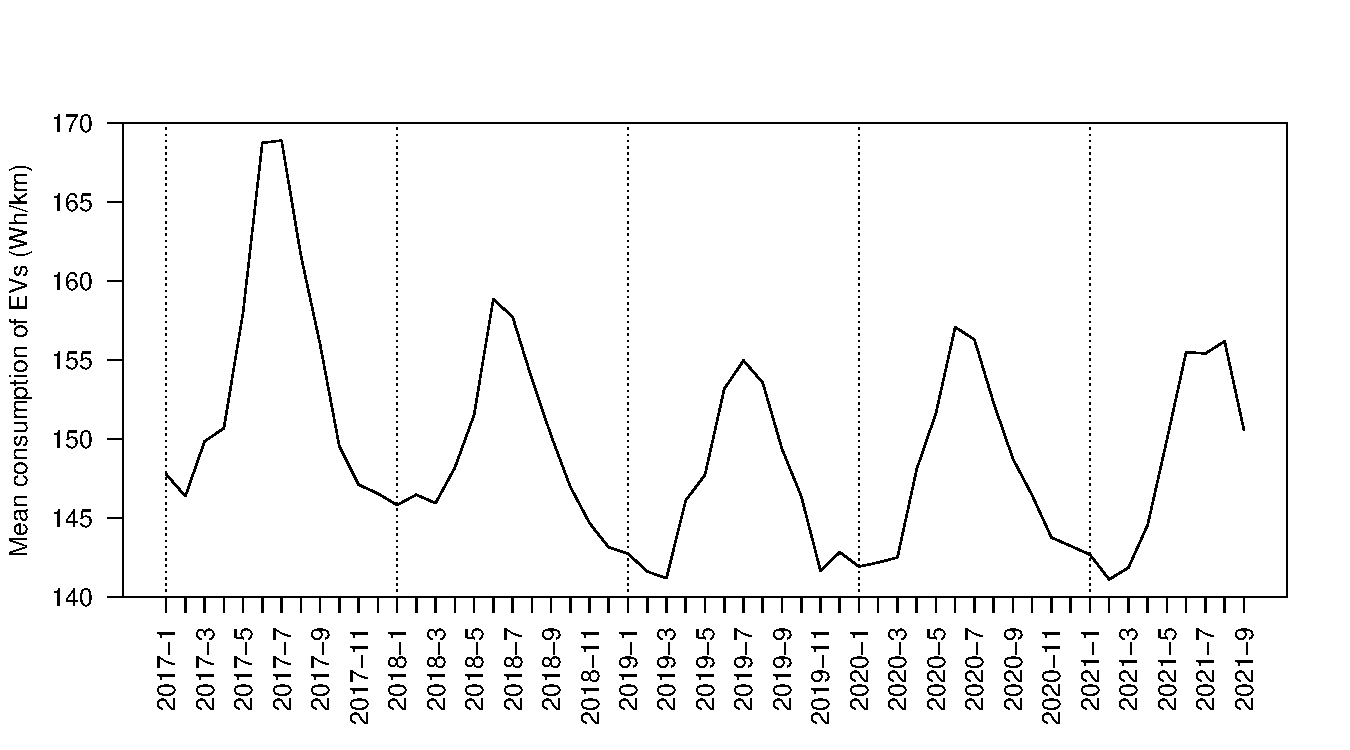
\includegraphics{summary_week4_files/figure-latex/eff_plot-1.pdf}
\caption{Time Series of EV Consumption}
\end{figure}

Plotting monthly average consumption of Flip the Fleets vehicles in all
of NZ we can see that there is a very clear seasonal trend.

\begin{comment}

  \begin{itemize}
    \item Linear model with each month as an independent factor
    \begin{itemize}
      \item offers more control and flexibility (could add vehicle type etc in further analysis)
      \item shows confidence interval
      \item requires to define an arbitrary function that can fit to the overall trend to separate from seasonal trend
      \item least squares is sensitive to single large deviation that could just be outlier (such as lockdown)
    \end{itemize}
    \item Time series Decomposition
    \begin{itemize}
      \item designed for time series
      \item automatically finds an overall trend based on the recent average to isolate the seasonal trend from
      \item less sensitive to a large deviation (such as lockdown) as attributed to noise compared to linear model
      \item no confidence interval
    \end{itemize}
  \end{itemize}
  
  In the end seems better to use Time series Decomposition for overall consumption trend but is still useful to see from the linear model without assuming any correlation between the months it still has very strong confidence intervals (p-value $< 2^{-16}$). Could be worth doing some more in depth using linear model and adding car as a factor.

\end{comment}

A time series Decomposition is used to isolated the seasonal trend in
consumption from the overall trend. This can be done for all regions of
NZ combined and also for each region independently.

\begin{figure}
\centering
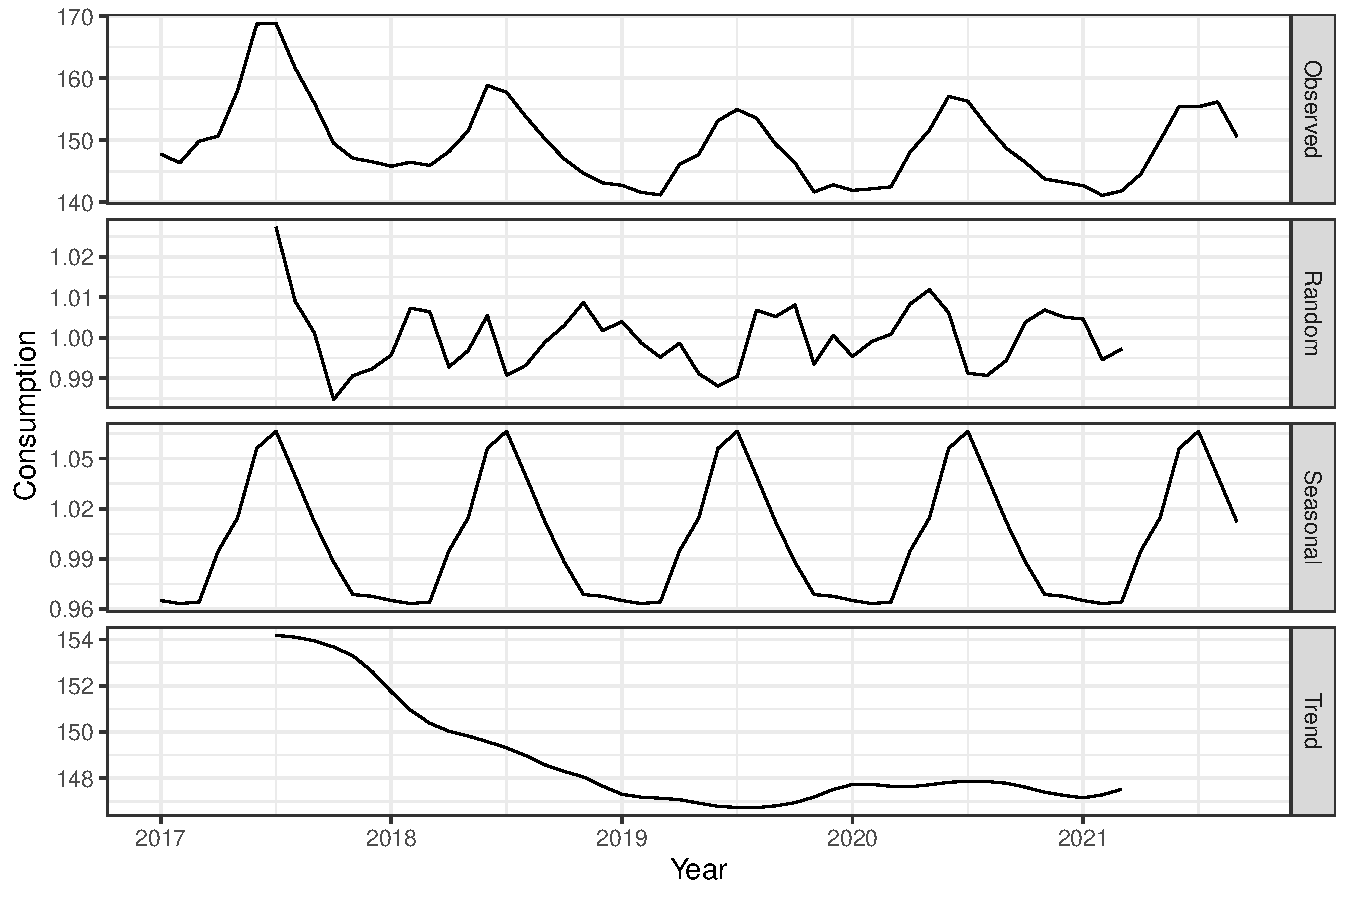
\includegraphics{summary_week4_files/figure-latex/consum_decomp_plot-1.pdf}
\caption{Multiplicative Time Series Decomposition of Flip the Fleet
Average Consumption for all of NZ\label{fig:consum_decomp_plot}}
\end{figure}

The decomposition shows that the seasonal trend goes from 0.96 times the
mean consumption in February to 1.07 times the mean consumption in
March, A peak to peak difference of 10.7\%.

Figure \ref{fig:consum_decomp_plot} shows a very clear seasonal trend
within the Flip the Fleets EV's consumption. As NZ weather differs
significantly by region, to test the hypothesis that EV consumption is
correlated with heating degree days we must limit the comparison to a
single region of Flip the Fleet data and its best corresponding weather
region. Auckland is used as an example in \ref{fig:eff_HDD_plot} as it
has the largest amount of data and is of most interest to Vector.

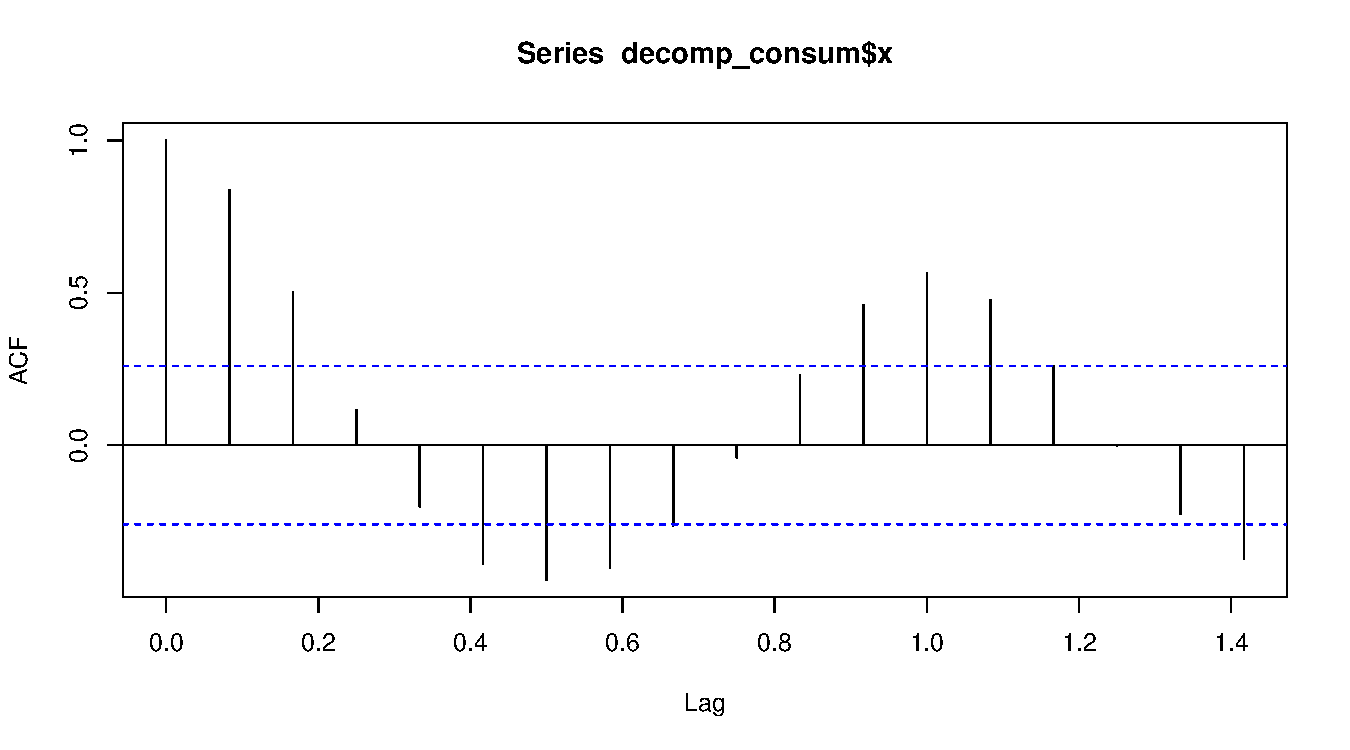
\includegraphics{summary_week4_files/figure-latex/unnamed-chunk-1-1.pdf}

\begin{figure}
\centering
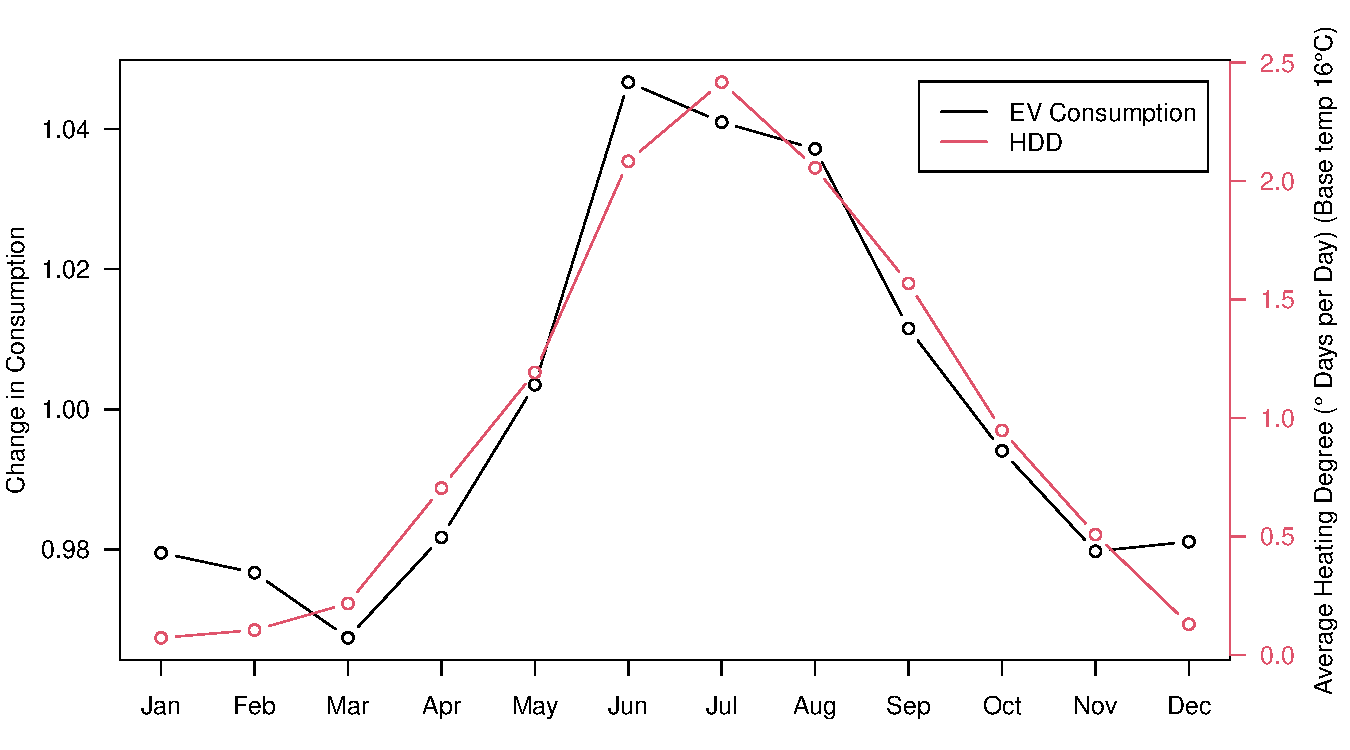
\includegraphics{summary_week4_files/figure-latex/eff_HDD_plot-1.pdf}
\caption{Auckland Seasonal component
Decompostions\label{fig:eff_HDD_plot}}
\end{figure}

Within Auckland looking at the plot it is very clear that HDD and
consumption of EVs are highly correlated. There is a slight increase in
consumption in January and February and it can be questioned if that is
due to AC usage which would decrease range \cite{ev_range} or other
factors such as holiday travel which could involve highway driving which
EVs are generally less efficient at \cite{ev_highway}. This effect is
not obvious in the overall trend this could be as Auckland for the most
part is a warmer climate than the rest of NZ.

\begin{figure}
\centering
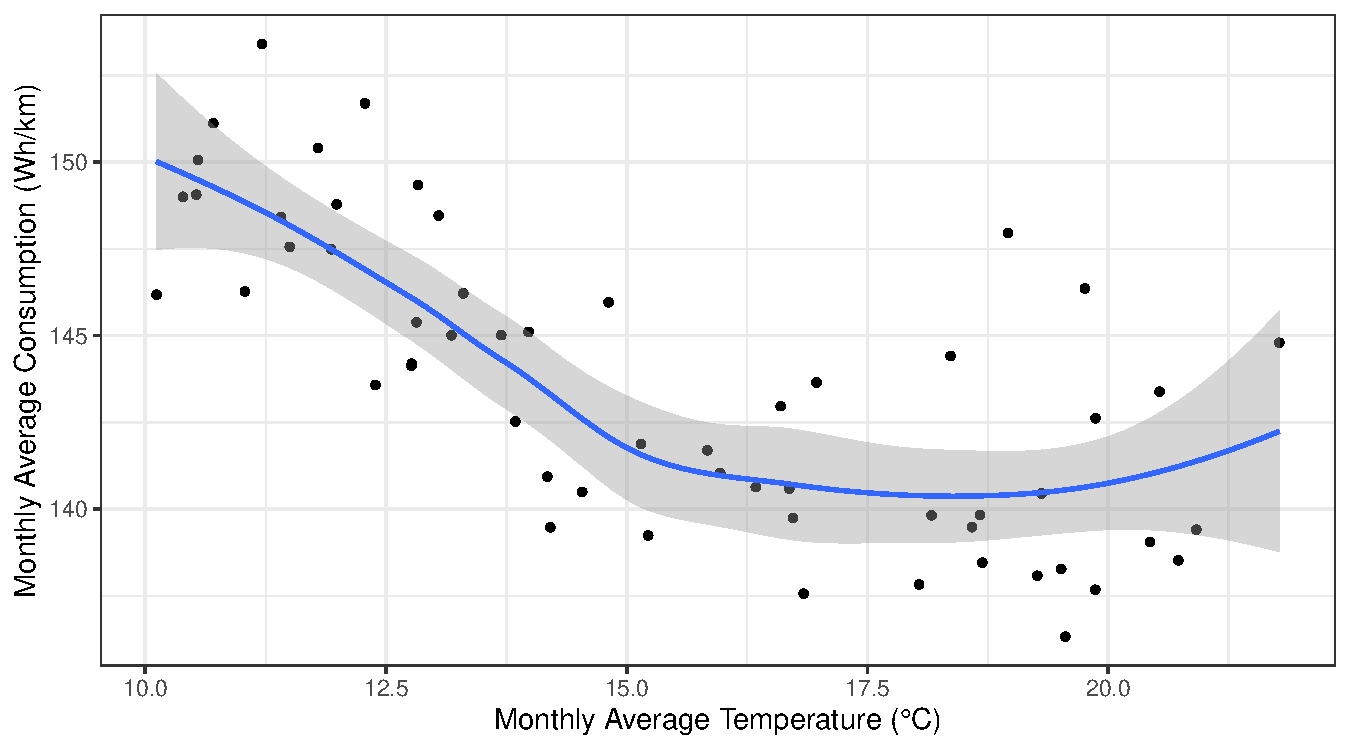
\includegraphics{summary_week4_files/figure-latex/temp_eff_plot-1.pdf}
\caption{Auckland Monthly Consumption by Temperature}
\end{figure}

Further looking into this we can see that in Auckland as the average
temperature of the month starts increasing past 17.5°C there appears to
be a trend towards increasing EV consumption. As stated before research
\cite{ev_range} suggested AC also increases consumption of the EV. This
suggest it may be worth including cooling degree days and heating degree
days in analysis. This could also be useful to explain the points well
above the trend line that may be from a month where there was both cold
and warm days contributing to a high usage of cabin temperature control
increasing consumption but average temperature would not be able to show
this.

\hypertarget{model}{%
\subsection{Model}\label{model}}

Due to this we propose using a linear model is used to model power
consumption by HDD and CDD given by the formula

\[ \eta = A_{CDD}{CDD} + A_{HDD}{HDD} + R + M + \epsilon\]

\[ \eta = A_{CDD}{CDD} + A_{HDD}{HDD} + B_{R,M} + \epsilon\]

As with the case of the adjusted monthly average power consumption
(Wh/km) in the linear model a weighting is added to the points in order
to give more weighting to cars with longer distance traveled. This may
give a slight bias towards EVs with proportionally higher highway
mileage. However, from the electricity grids perspective it makes sense
to give less weighting to cars that have traveled 0 or very low km.
Mathematically this means instead of estimating the coefficients by
minimizing the RSS given by the function
\(\sum_{i =1}^{n}(y_{i}-\hat{y}_{i})^2\) we minimize the function
\(\sum_{i =1}^{n}d \cdot(y_{i}-\hat{y}_{i})^2\) where \(d\) is the
distance traveled by a car in that month, \(y_{i}\) is the actual power
consumption, and \(\hat{y}_{i}\) is the power consumption of that
vehicle as predicted by the model.

Power consumption is used in conjunction with a linear model as with the
correct base temperature the usage of power to warm/cool the cabin
should be roughly linear to the HDD/CDD \cite{HDD_est}. This would allow
energy used to heat/cool the car to be isolated for analysis from
drivetrain power consumption. Conceptually it makes sense that extra
power usage due to heating/cooling demand to be independent from
drivetrain demand as unlike in traditional internal combustion engine
(ICE) vehicles where the energy to heat and cool the cabin comes from
the engine, an EVs heat pump and AC can draw power independently from
the engine. Unfortunately, this linear correlation may break down as
cars unlike houses or buildings are often only used at particular hours
of the day for short periods so this may break down or have more
dependency towards the temperature at times such as the morning or
evening commute hours.

A different intercept is used for each model of car as a majority of the
variation in efficiency will be due to different vehicle models,
therefore, including the vehicle model allows for much better model fit
and smaller confidence intervals. A different intercept is also used for
each weather region as weather might be measured in a cold or hot
section of region and also the region may have more or less hill/highway
which could influence driving patterns impacting efficiency (for
simplicity preferable if not included but model is much better fit if is
included). However the Gradient of HDD term and CDD term is kept same
for all regions and models as this is the number we are trying to find
to see how the number of HDD and CDD affect the efficiency of the EV. A
baseline of Auckland and Nissan Leaf (24 kWh) 2013-2016 are used for the
region and model as there is the most amount of data in them.

\begin{longtable}[]{@{}
  >{\raggedright\arraybackslash}p{(\columnwidth - 8\tabcolsep) * \real{0.41}}
  >{\raggedleft\arraybackslash}p{(\columnwidth - 8\tabcolsep) * \real{0.14}}
  >{\raggedleft\arraybackslash}p{(\columnwidth - 8\tabcolsep) * \real{0.16}}
  >{\raggedleft\arraybackslash}p{(\columnwidth - 8\tabcolsep) * \real{0.12}}
  >{\raggedleft\arraybackslash}p{(\columnwidth - 8\tabcolsep) * \real{0.16}}@{}}
\toprule
\begin{minipage}[b]{\linewidth}\raggedright
~
\end{minipage} & \begin{minipage}[b]{\linewidth}\raggedleft
Estimate
\end{minipage} & \begin{minipage}[b]{\linewidth}\raggedleft
Std. Error
\end{minipage} & \begin{minipage}[b]{\linewidth}\raggedleft
t value
\end{minipage} & \begin{minipage}[b]{\linewidth}\raggedleft
Pr(\textgreater\textbar t\textbar)
\end{minipage} \\
\midrule
\endhead
(Intercept) & 132.1 & 0.2867 & 460.8 & 0 \\
HDD & 2.195 & 0.05096 & 43.07 & 0 \\
CDD & 2.347 & 0.5722 & 4.102 & 4.113e-05 \\
weather\_regionUpper Hutt & -0.4796 & 0.3036 & -1.58 & 0.1141 \\
weather\_regionChristchurch & -0.9073 & 0.3257 & -2.786 & 0.005348 \\
weather\_regionDunedin & 12.06 & 0.3835 & 31.45 & 1.705e-212 \\
weather\_regionHamilton & 8.513 & 0.5298 & 16.07 & 8.999e-58 \\
weather\_regionNelson & 2.711 & 0.4806 & 5.642 & 1.7e-08 \\
weather\_regionRotorua & 5.015 & 0.5462 & 9.182 & 4.597e-20 \\
weather\_regionClyde & 4.53 & 0.7491 & 6.048 & 1.494e-09 \\
weather\_regionPalmerston North & 14.11 & 0.6652 & 21.21 & 6.519e-99 \\
weather\_regionStratford & 10.36 & 0.9497 & 10.91 & 1.254e-27 \\
weather\_regionNapier & 6.316 & 0.8473 & 7.455 & 9.311e-14 \\
weather\_regionInvercargill & 3.191 & 1.758 & 1.815 & 0.06949 \\
modelNissan Leaf (30 kWh) & 3.401 & 0.2524 & 13.47 & 3.276e-41 \\
modelNissan Leaf (24 kWh) 2011-2012 & 12.39 & 0.3246 & 38.17 &
7.229e-309 \\
modelNissan Leaf (40 kWh) & 10.68 & 0.5174 & 20.63 & 1.046e-93 \\
modelNissan e-NV200 (24 kWh) & 32.71 & 0.5367 & 60.95 & 0 \\
modelHyundai Ioniq (EV) & -18.32 & 0.685 & -26.75 & 3.342e-155 \\
modelBMW i3 & -1.335 & 0.7873 & -1.695 & 0.09006 \\
modelHyundai Kona (EV) & 0.6822 & 0.86 & 0.7933 & 0.4276 \\
modelRenault Zoe & 11.55 & 0.8507 & 13.57 & 8.383e-42 \\
modelTesla Model 3 & 10.55 & 1.022 & 10.32 & 6.485e-25 \\
modelNissan Leaf (62 kWh) & 25.46 & 1.752 & 14.53 & 1.295e-47 \\
modelKia Niro (EV) & 11.34 & 1.193 & 9.511 & 2.075e-21 \\
modelTesla Model S & 48.38 & 1.69 & 28.63 & 4.806e-177 \\
modelVolkswagen e-Golf & 1.208 & 1.538 & 0.7853 & 0.4323 \\
modelTesla Model-X & 104.1 & 1.296 & 80.34 & 0 \\
modelKia Soul & 6.276 & 1.25 & 5.022 & 5.15e-07 \\
modelMG ZS EV & 22.12 & 3.9 & 5.671 & 1.439e-08 \\
modelRenault Kangoo (van) & 56.63 & 1.537 & 36.84 & 1.301e-288 \\
modelJaguar I-PACE & 73.02 & 2.951 & 24.75 & 1.949e-133 \\
modelPeugeot e-208 & 10.96 & 9.581 & 1.144 & 0.2525 \\
\bottomrule
\end{longtable}

\begin{longtable}[]{@{}
  >{\raggedleft\arraybackslash}p{(\columnwidth - 6\tabcolsep) * \real{0.21}}
  >{\raggedleft\arraybackslash}p{(\columnwidth - 6\tabcolsep) * \real{0.31}}
  >{\raggedleft\arraybackslash}p{(\columnwidth - 6\tabcolsep) * \real{0.12}}
  >{\raggedleft\arraybackslash}p{(\columnwidth - 6\tabcolsep) * \real{0.24}}@{}}
\caption{Fitting linear model: consumption \textasciitilde{} HDD + CDD +
weather\_region + model}\tabularnewline
\toprule
\begin{minipage}[b]{\linewidth}\raggedleft
Observations
\end{minipage} & \begin{minipage}[b]{\linewidth}\raggedleft
Residual Std. Error
\end{minipage} & \begin{minipage}[b]{\linewidth}\raggedleft
\(R^2\)
\end{minipage} & \begin{minipage}[b]{\linewidth}\raggedleft
Adjusted \(R^2\)
\end{minipage} \\
\midrule
\endfirsthead
\toprule
\begin{minipage}[b]{\linewidth}\raggedleft
Observations
\end{minipage} & \begin{minipage}[b]{\linewidth}\raggedleft
Residual Std. Error
\end{minipage} & \begin{minipage}[b]{\linewidth}\raggedleft
\(R^2\)
\end{minipage} & \begin{minipage}[b]{\linewidth}\raggedleft
Adjusted \(R^2\)
\end{minipage} \\
\midrule
\endhead
22592 & 492.2 & 0.4855 & 0.4848 \\
\bottomrule
\end{longtable}

The HDD term suggests that as the average number of heating degree days
per days increases by 1 the average power consumption of EVs for the
month increases by 2.19Wh/km. With a p-value of \(<2\times10^{-16}\) we
are quite confident on this value.

The CDD term suggests that as the average number of cooling degree days
per days increases by 1 the average power consumption of EVs for the
month increases by 2.35Wh/km. With a p-value of \(4.11\times10^{-5}\) we
are less confident on this value. This is likely as there is much less
data in New Zealand regarding cooling degree days as NZ is a much cooler
climate compared to where a lot of the other research on EVs is going
on.

If we know that EVs have higher consumption in the winter due to heating
requirements and to a much lesser extent in NZ higher consumption on
warm days due to AC in order to see how this will affect the grid we
need to see how this correlates with NZ populations driving pattern.

For now I have 3 data sets regarding fuel usage

\begin{itemize}
  \item monthly card sales data 
  \begin{itemize}
    \item monthly data for all of NZ credit card transactions at fuel stations
  \end{itemize}
  \item quarterly regional fuel sales data
  \begin{itemize}
    \item quarterly data for all sales at fuel stations broken down by region from MBIE
  \end{itemize}
  \item quarterly fuel trade data
    \begin{itemize}
    \item quarterly data of fuel used for transport by type of fuel
  \end{itemize}
\end{itemize}

As an initial analysis of the fuel usage in NZ I load the quarterly fuel
trade data so that I can isolate only petrol usage in domestic land
transport which should be an accurate representation of the fuel usage
by light passenger vehicles. Will be just combining regular petrol and
premium for analysis. (Premium used to be more popular. Was there a
definition change on premium and regular used in the data?)

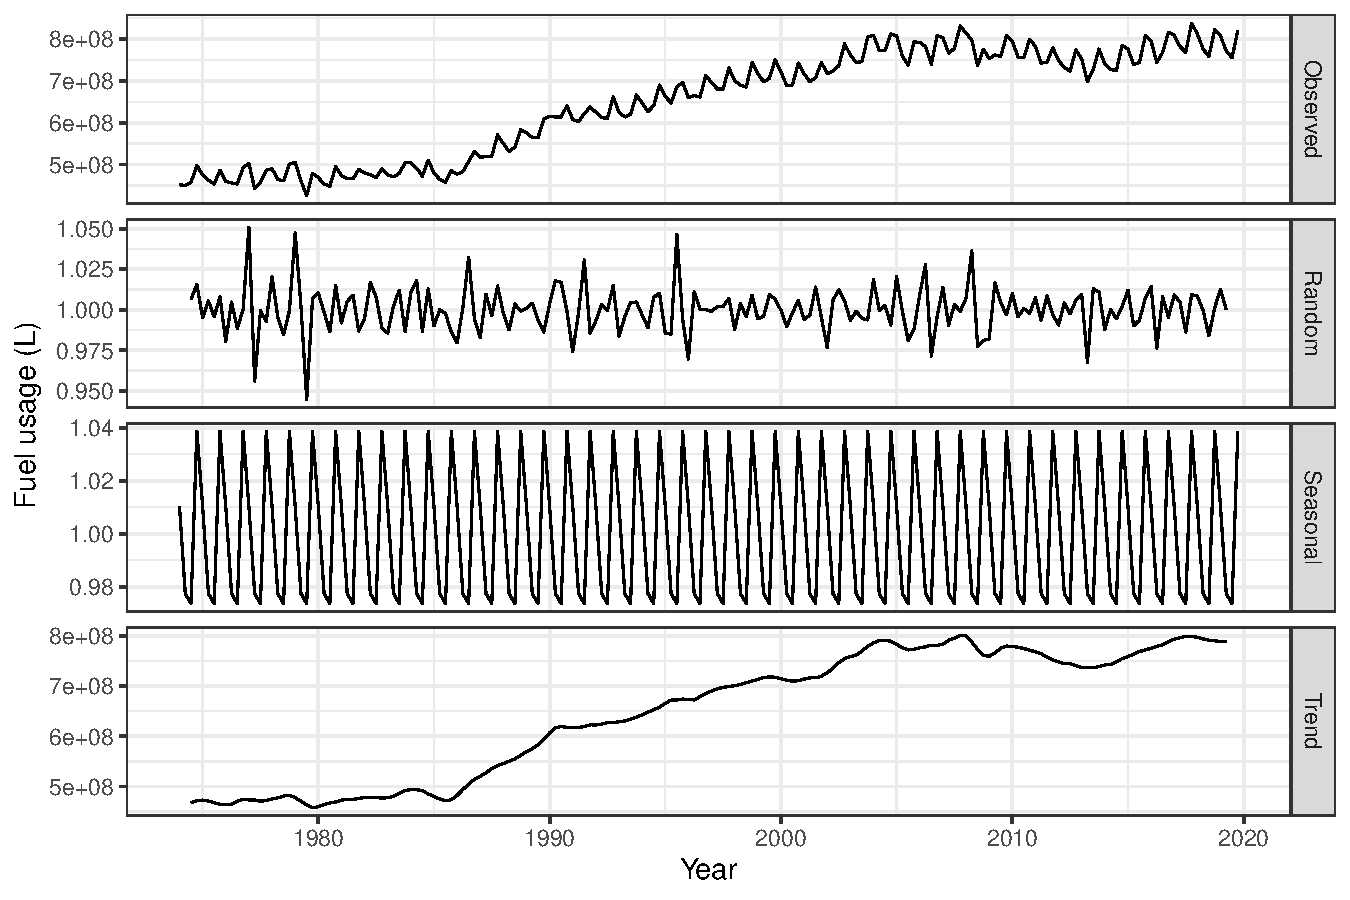
\includegraphics{summary_week4_files/figure-latex/petrol_ts-1.pdf}
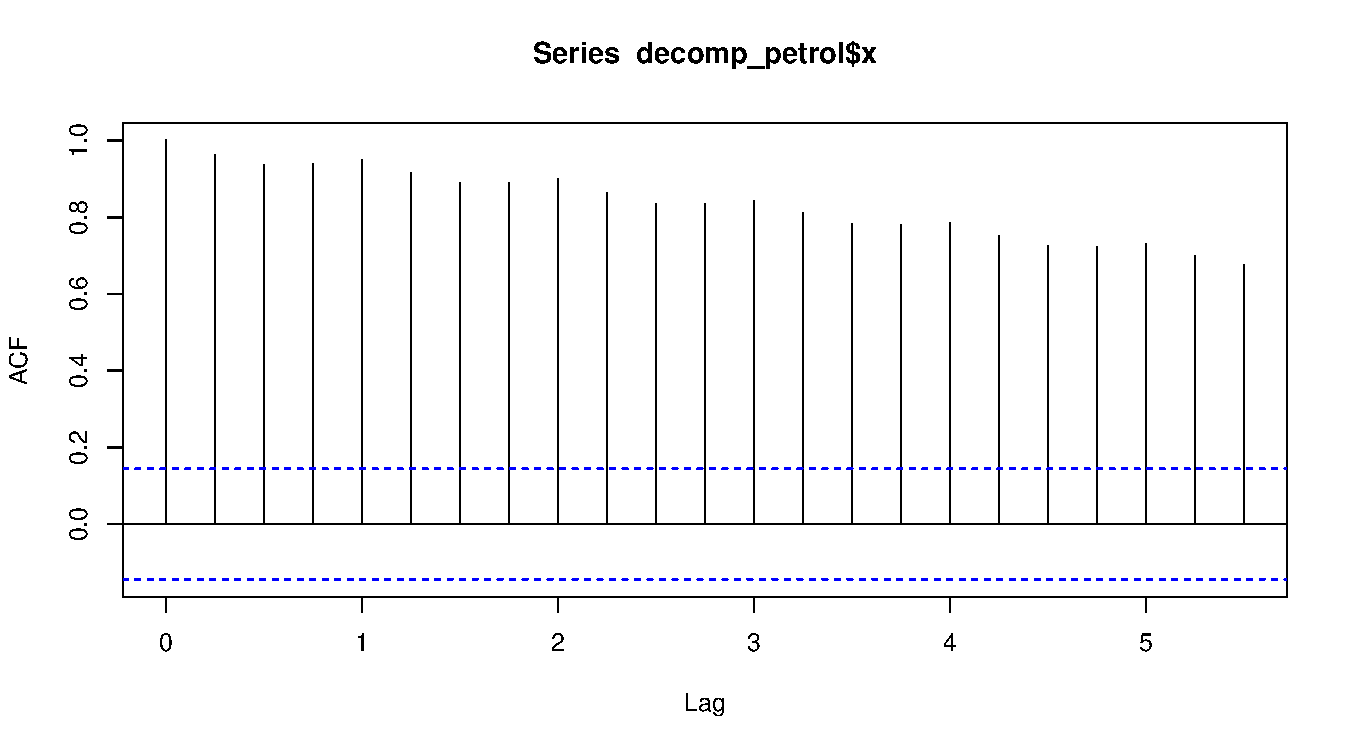
\includegraphics{summary_week4_files/figure-latex/unnamed-chunk-2-1.pdf}

Fuel trade data from 2020 was excluded as lockdowns were not an accurate
representation of the general driving patterns of the NZ population.
Looking at the decomposition above there is a clear seasonal trend
however it not that significant and is smaller than the larger
deviations of the random variations.

Fuel trade data can be compared to the VKT data from NZTA. This data was
given by Haobo Wang from NZTA and is collected using VKT based on
WoF/CoF odometer \cite{NZTA_VKT}.

\begin{figure}
\centering
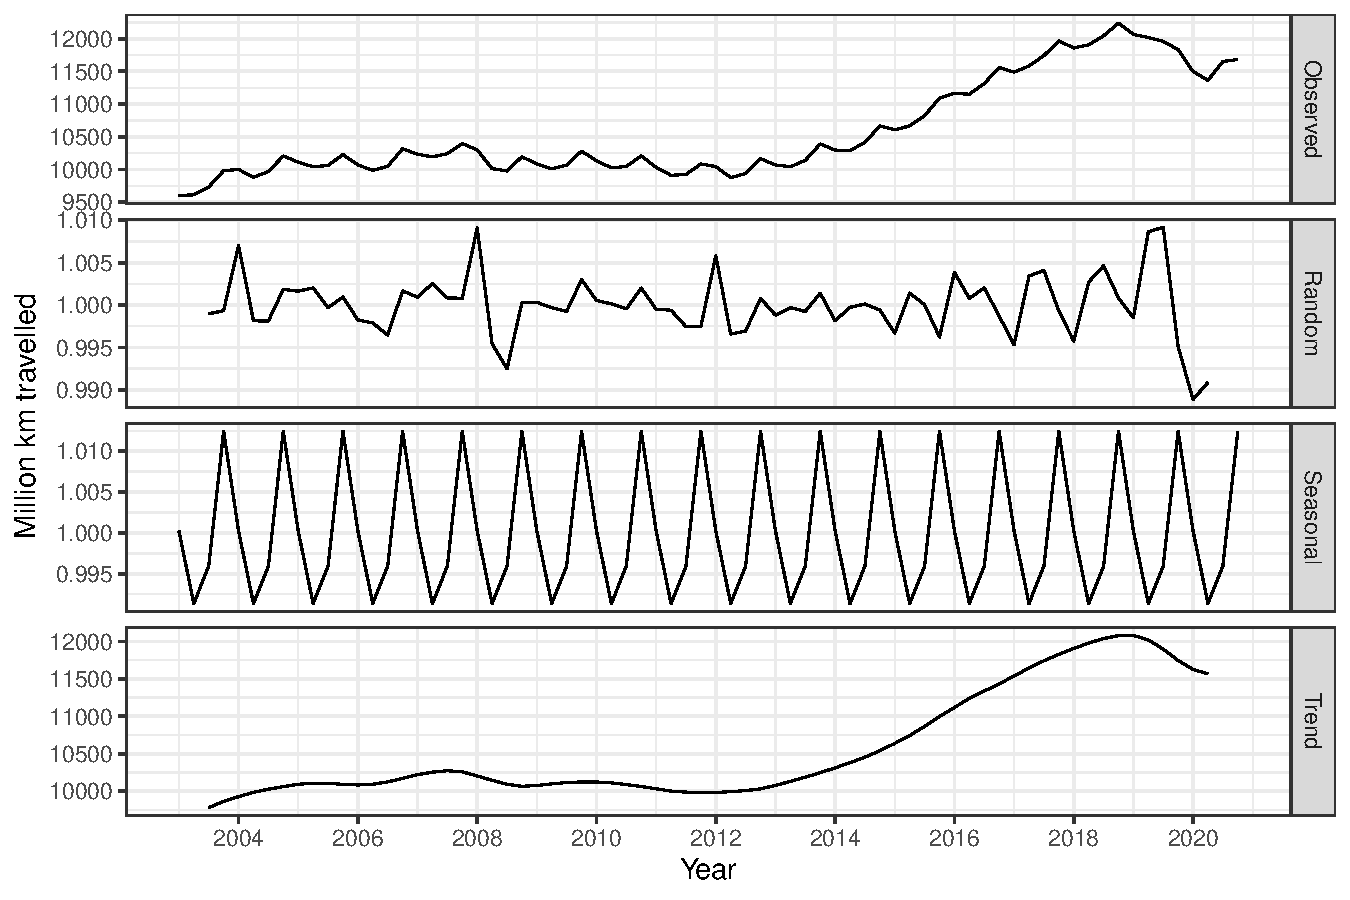
\includegraphics{summary_week4_files/figure-latex/VKT_ts-1.pdf}
\caption{Decomposition of NZ VKT Time Series}
\end{figure}

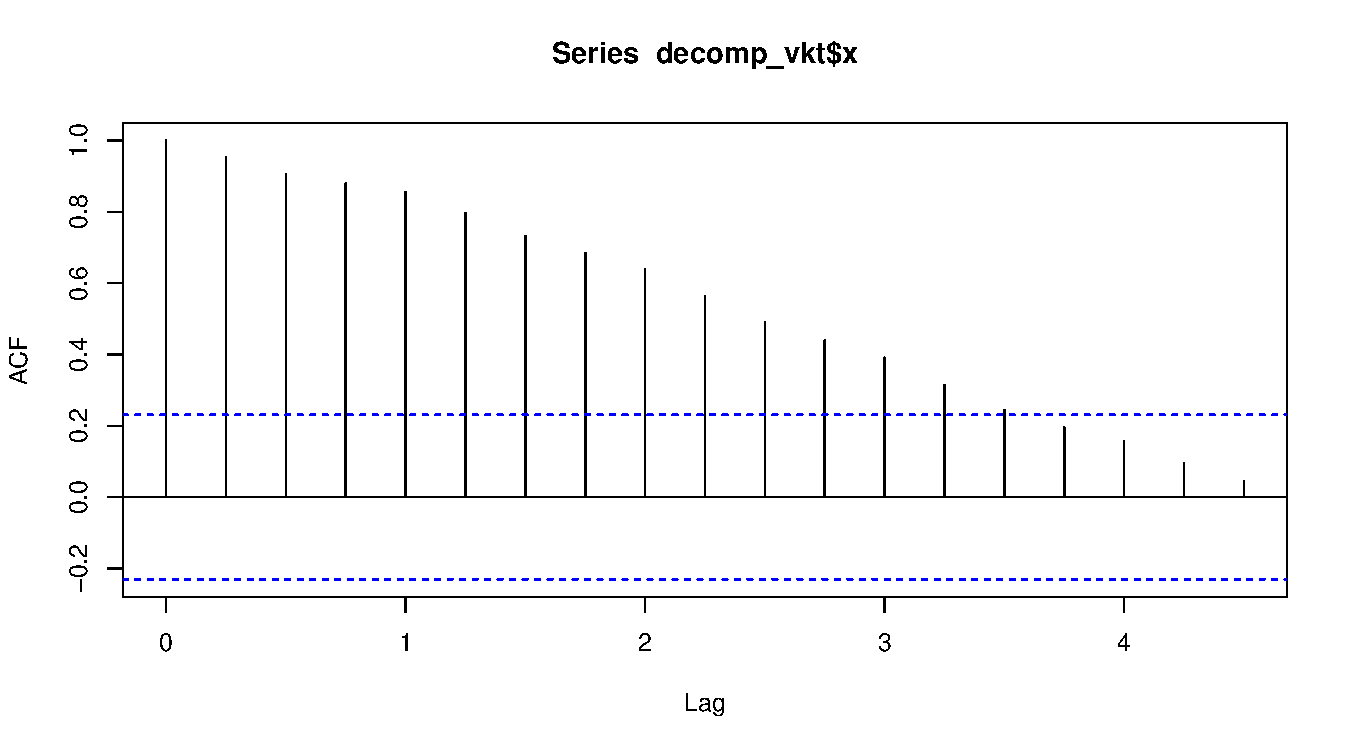
\includegraphics{summary_week4_files/figure-latex/unnamed-chunk-3-1.pdf}

The time series decomposition of the NZ VKT data shows a clear seasonal
trend, albeit smaller than the trend from the fuel sales data. There is,
however, clearly a large amount of smoothing going on with this data.
This is shown in a couple of different ways including.

\begin{itemize}
\item The drop of VKT due to lockdown which started in 2020 March is already visible in the data from early 2019. 
\item Related to the previous point, the Random component of Time Series Decomposition shows only a 10\% decrease in VKT spread out over a 1 year period from lockdown compared to 30\% drop in fuel usage only during 1 quarter shown in the MIBE fuel trade data. 
\item Random variation in MIBE fuel trade data shows around a 3 times greater random variation. There could be a seasonal effect on fuel efficiency which could change seasonal fuel trend relative to VKT but there is no reason there would be any randomness in fuel efficiency so randomness should be of similar magnitude.
\end{itemize}

This smoothing likely occurs due to the method of data collection using
the odometer readings during WoF/CoF. For a majority of vehicles WoF is
only done once a year and in the case of new cars that could be up to 3
years. This likely causes the data to show less seasonal trend than may
exist in the real world.

Looking at the long term trend VKT remained largely flat between 2004
and 2012 after which there was a steady but significant increase until
2019. After which there is a decrease in VKT due to lockdown, which in
this data set for the above reasons likely started showing its effects
in 2019.

\begin{figure}
\centering
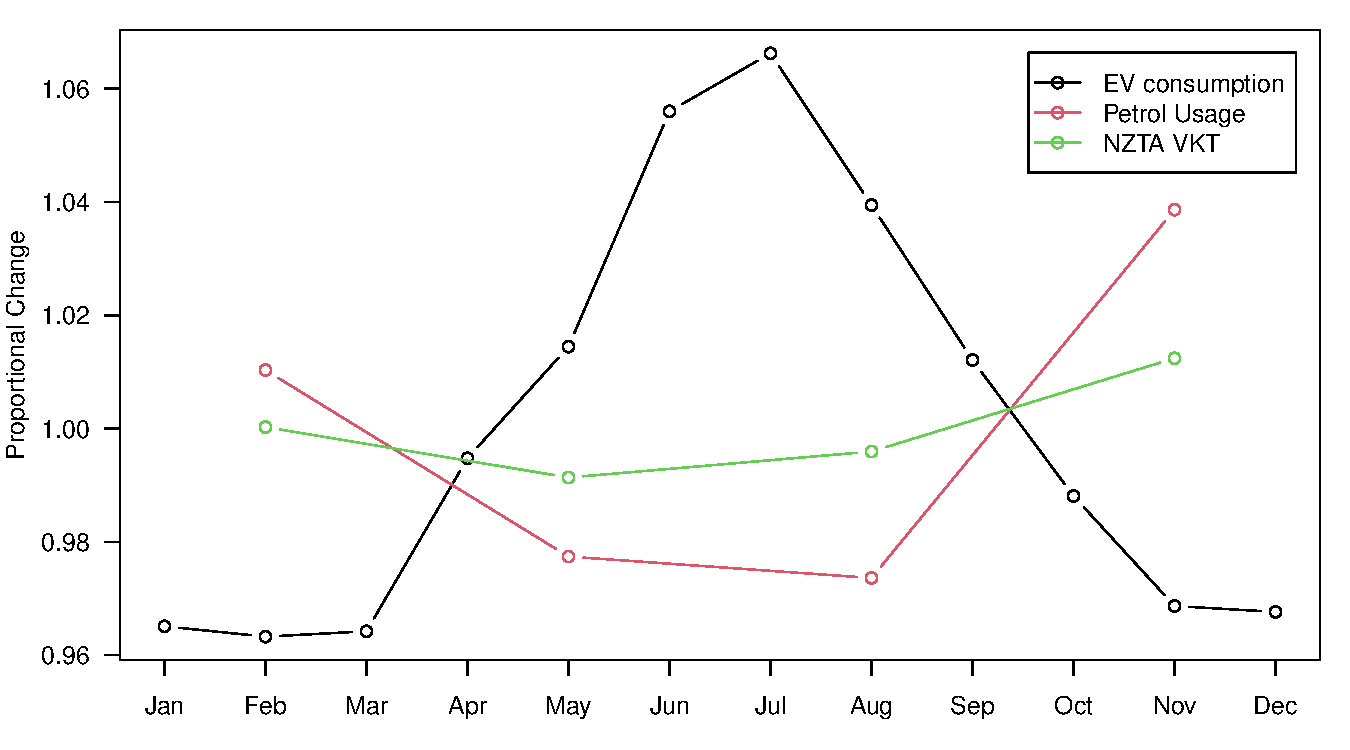
\includegraphics{summary_week4_files/figure-latex/petrol_VKT_vs_eff-1.pdf}
\caption{NZ Seasonal Component Decompostions}
\end{figure}

Looking at the Seasonal trend of Petrol Usage and VKT data from NZTA we
can see an obvious decrease in the winter months with a peak in the 4th
quarter likely corresponding to holiday travel. Petrol Usage shows this
variation to be much larger than the VKT data from NZTA. It is unclear
whether this would be due to the smoothing effect as was previously
discussed on the NZTA data or perhaps a change in efficiency for petrol
vehicle by seasons similar to that of the EV. However if this was a
seasonal effect it is odd that the increase in petrol usage occurs in
4th quarter rather than the 1st quarter, as the 1st quarter is generally
warmer than the 4th quarter, as shown by the EV efficiency increasing
more significantly in 1st quarter than 4th quarter. Combining these 2
data sets it is reasonable to suggest that in New Zealand, compared to
the winter (Q2 and Q3) VKT, the true VKT in the summer (Q1 and Q4) is
between 1.3\% higher, as suggested by the VKT data from NZTA, to 5\%
higher, according to the petrol usage data.

Looking at the seasonal trend of EV consumption we can see much larger
increase in consumption in the winter months with average consumption in
July being 10.7\% higher consumption than in February. From the plot we
can see that when consumption of EVs increases, VKT goes down,
suggesting that some increase in total power usage due to EVs increase
in consumption will be countered by the decrease in VKT. However, the
increase in consumption is much larger than than the decrease in VKT.
This combined with the fact that winter is when our electricity grid in
New Zealand is already under strain due to heating demand suggests that
if we ignore the relatively small change in VKT in our model we can
effectively model a worst case scenario.

In order to predict the the effect that EVs will have on New Zealands
electricity grid the yearly regional VKT data from 2019 in used in
conjunction with the consumption linear model from above, with weather
data from 2017 to 2021 matched to the best corresponding VKT regions and
the vehicle model make up of the Flip the Fleet data.

\hypertarget{predictions}{%
\subsection{Predictions}\label{predictions}}

Assumptions made are therefore,

\begin{itemize}
\item Regional VKT data remains relatively consistent with 2019 VKT data. 2019 is chosen as in NZ there has been a significant increase in VKT in recent years excluding 2020 as there was a significant decrease due to lockdown. As lockdown is an outlier event it would be preferable to not include this in the model so 2019 is used.
\item Regional weather data from 2017 to 2021 remains consistent with future climate of NZ.
\item Flip the Fleet's fleet is representative NZs future EV fleet.
\item Actual VKT of each region remains relatively constant throughout the year.
\end{itemize}

\begin{figure}
\centering
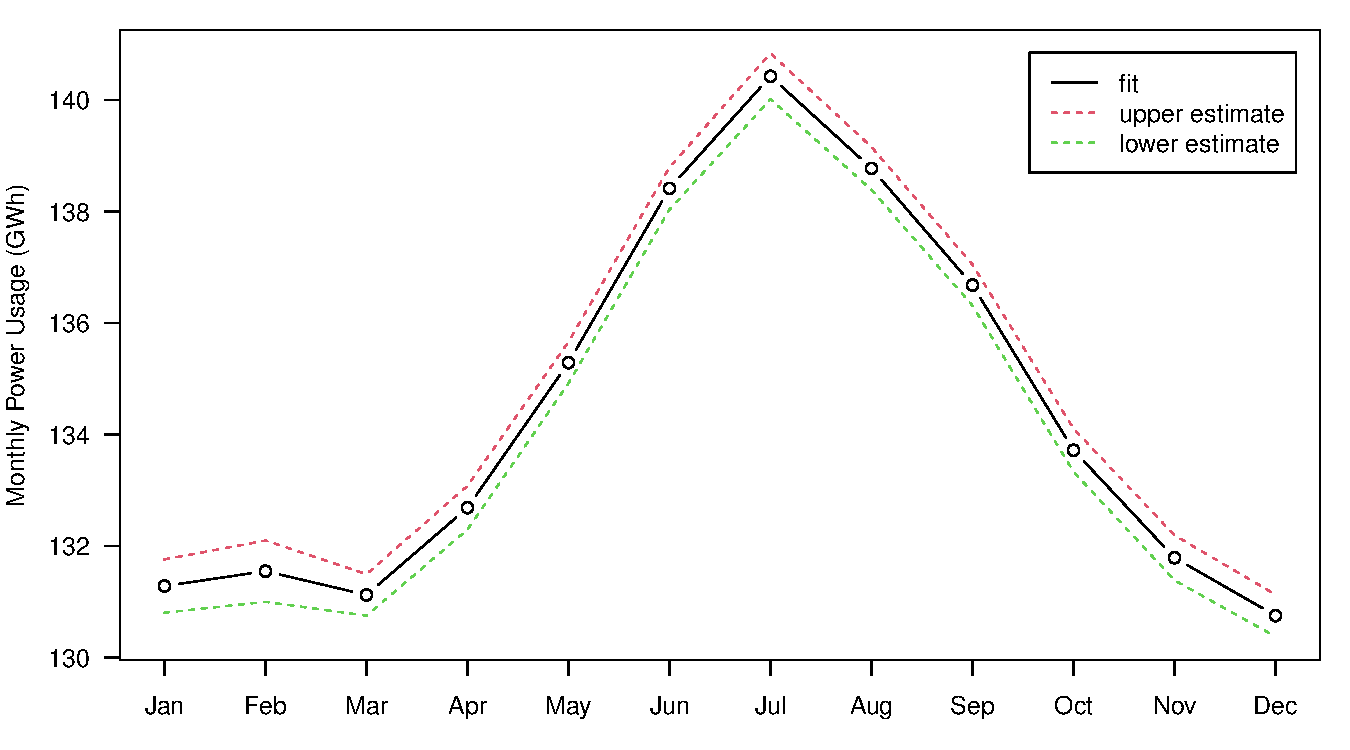
\includegraphics{summary_week4_files/figure-latex/Auckland_power-1.pdf}
\caption{Auckland Region 100\% EV Case Total Power Usage per Month}
\end{figure}

Combining Auckland only VKT with the consumption linear model we can see
the estimated power usage per month showing a clear seasonal trend from
around 130.8 GWh per month in summer to around 140.4 GWh per month in
the winter.

The upper and lower estimate are 95\% confidence interval on the linear
model. As confidence intervals are unknown for the future VKT and future
weather the confidence intervals do not include this uncertainty.
(should i just remove from the plot as do not have much meaning)

\begin{figure}
\centering
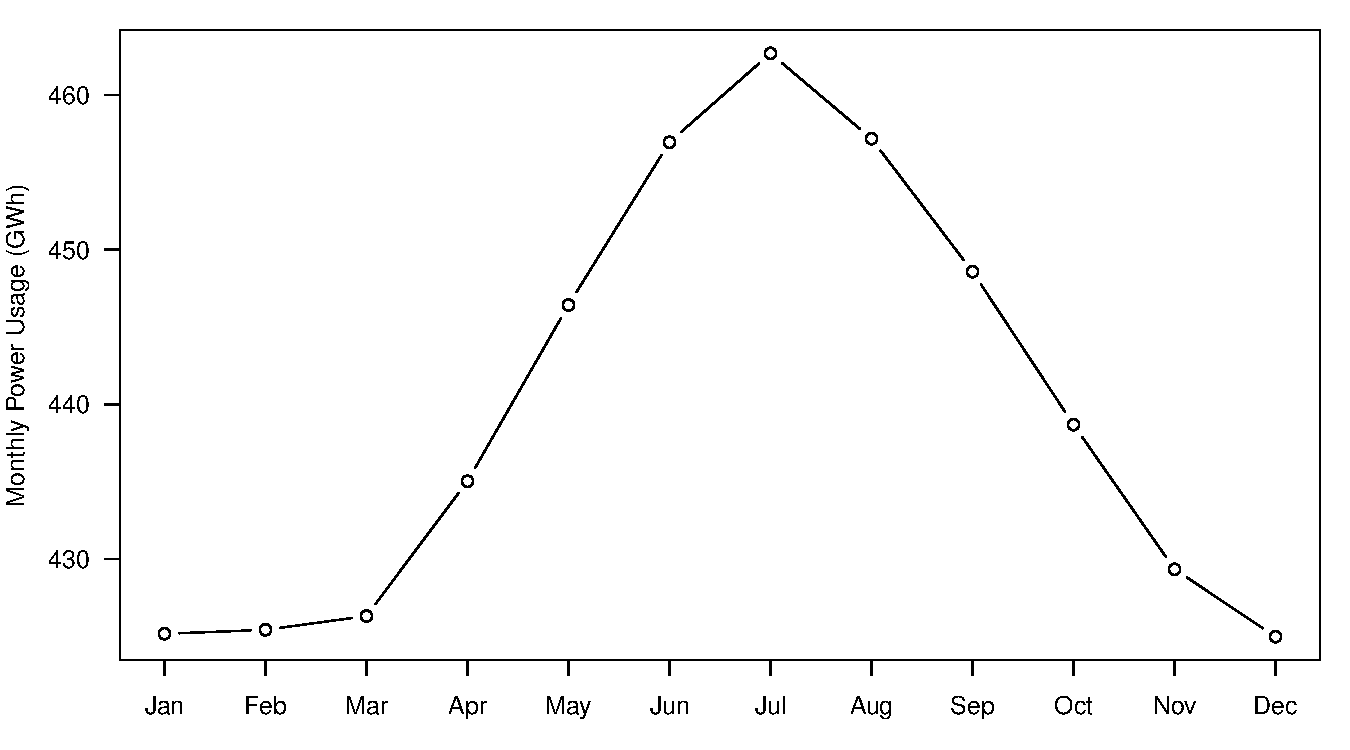
\includegraphics{summary_week4_files/figure-latex/NZ_power-1.pdf}
\caption{NZ 100\% EV Case Total Power Usage per Month}
\end{figure}

Similarly for all of NZ each VKT region is combined with the consumption
linear model for each best corresponding weather region. Again estimated
power usage per month is showing a clear seasonal trend from around 425
GWh per month in summer to around 463 GWh per month in the winter.

\begin{figure}
\centering
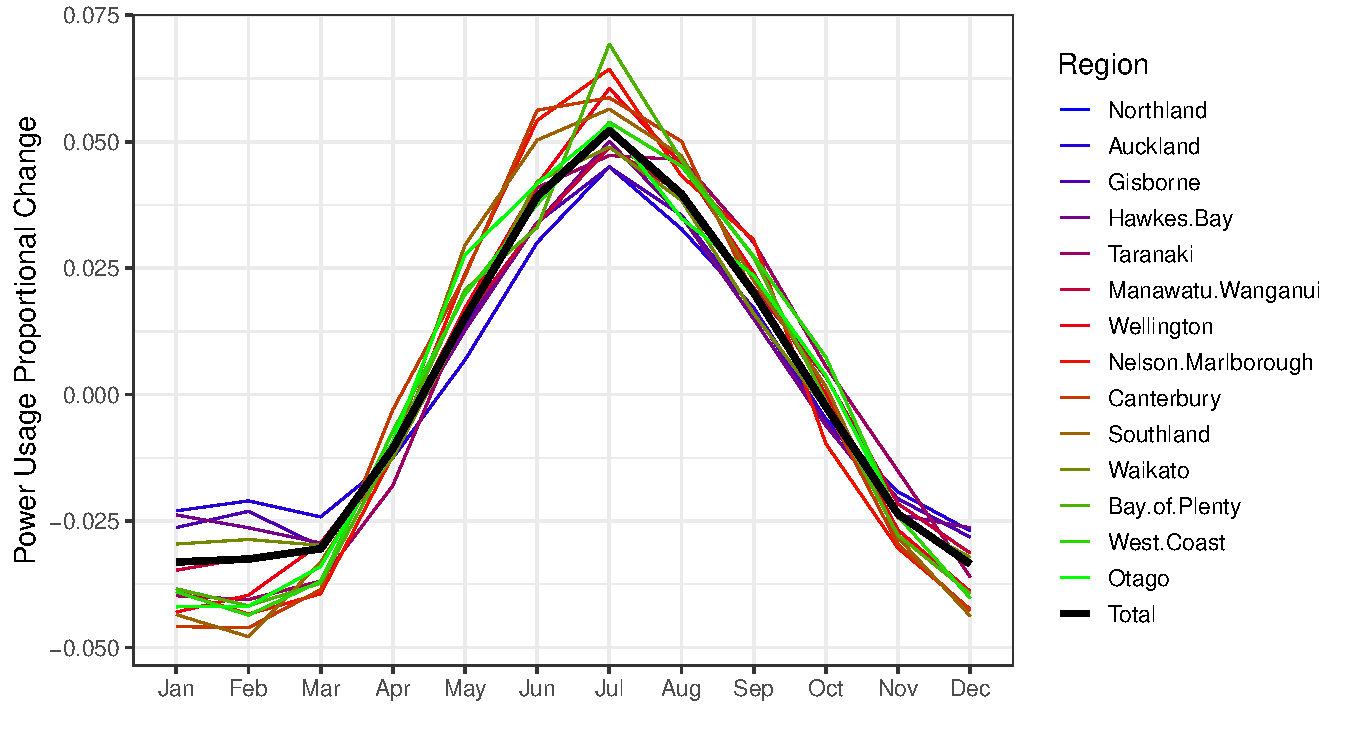
\includegraphics{summary_week4_files/figure-latex/NZ_region_power_prop-1.pdf}
\caption{All NZ Regions Monthly Proportional Change in Power Usage
Relative to its Yearly Average}
\end{figure}

Using the weather data only we can see the proportional change in power
usage for each region in NZ. All regions follow a similar seasonal
change in power consumption. Of note regions like Northland and Auckland
appear to have less of a seasonal trend compared to regions such as
Otago and the West Coast likely due to a warmer climate leading to
increased AC usage during the summer months decreasing efficiency in the
summer month.

\begin{figure}
\centering
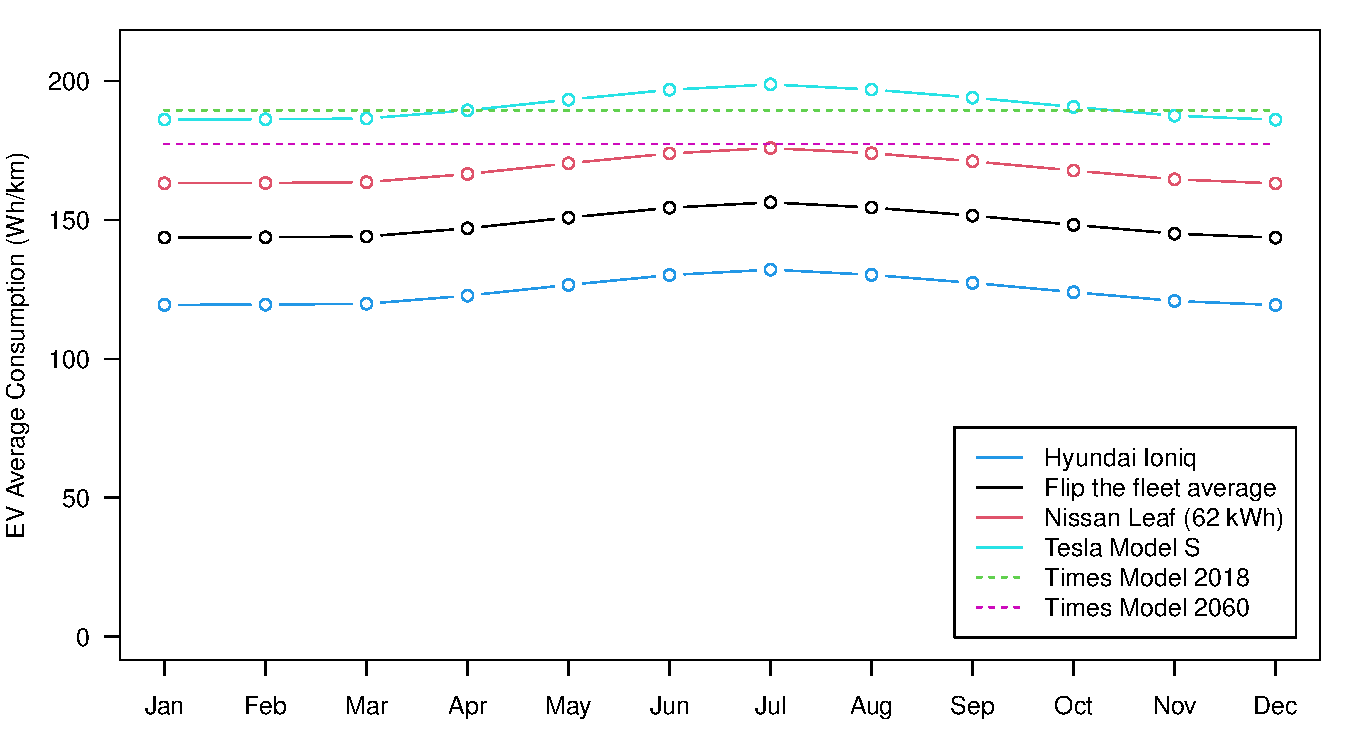
\includegraphics{summary_week4_files/figure-latex/vehicle_consum-1.pdf}
\caption{NZ Vehicle Average Consumption
Scenarios\label{fig:vehicle_consum}}
\end{figure}

Comparing flip the fleet consumption numbers to EECA's times tui model
\cite{times_model} consumption we can see that ECCA's times model is
based on a much higher consumption (lower efficiency) than the flip the
fleet data would suggest. With the consumption model using the flip the
fleet vehicle make up suggests an average of 148.6Wh/km. However, this
is consisting of primarily of Nissan leafs with 1078 out of 1264
vehicles included in the flip the fleet data being Nissan leafs which is
a quite light and efficient EV. The 2018 times model consumption is much
more comparable to much heavier and less efficient Tesla Model S (based
on 81 months of efficiency data from 5 vehicles).

Figure \ref{fig:vehicle_consum}, while showing a seasonal trend, shows
that the vehicle make up of the fleet can have a much greater impact
than anything else on the actual power consumption that EVs will have on
the power grid.

\begin{figure}
\centering
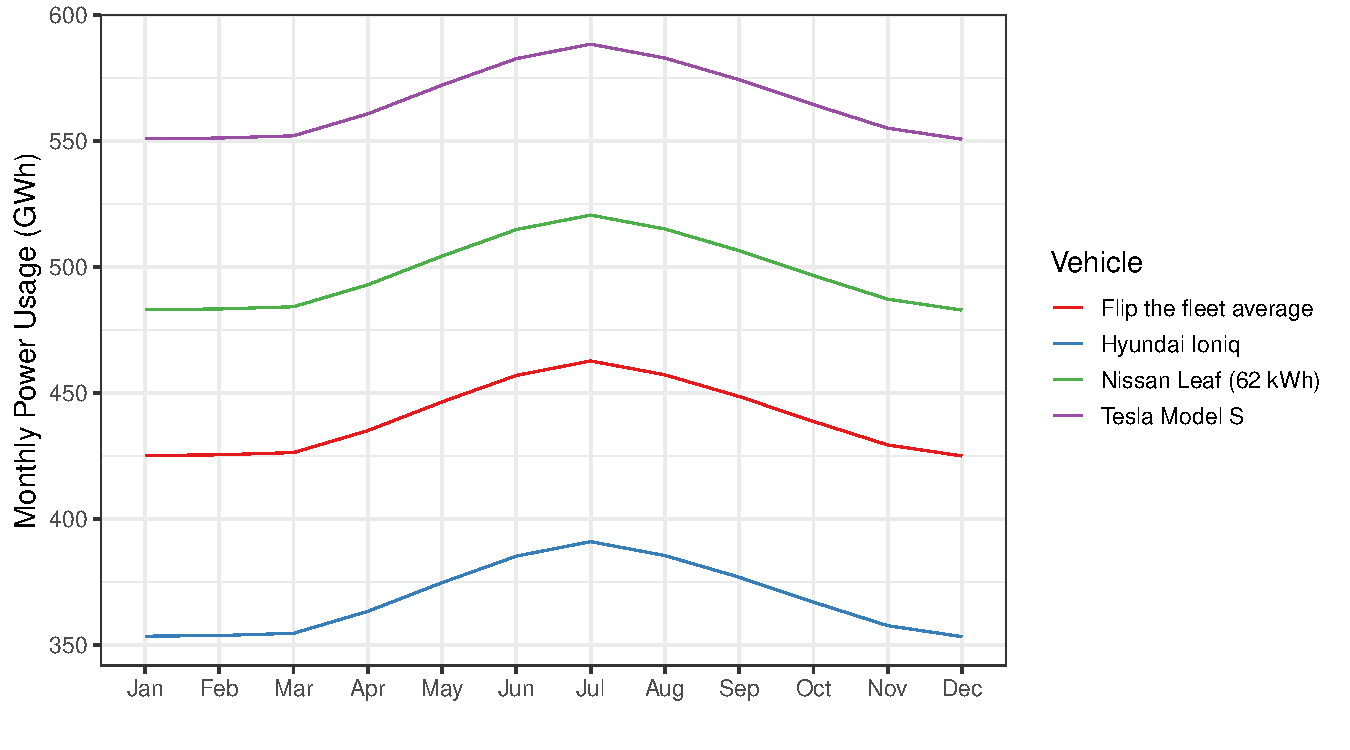
\includegraphics{summary_week4_files/figure-latex/vehicle_power_usage-1.pdf}
\caption{2019 VKT 100\% EV Case NZ Total Power Usage Scenarios by
Vehicle Fleet Model Makeup\label{fig:vehicle_power_usage}}
\end{figure}

\begin{figure}
\centering
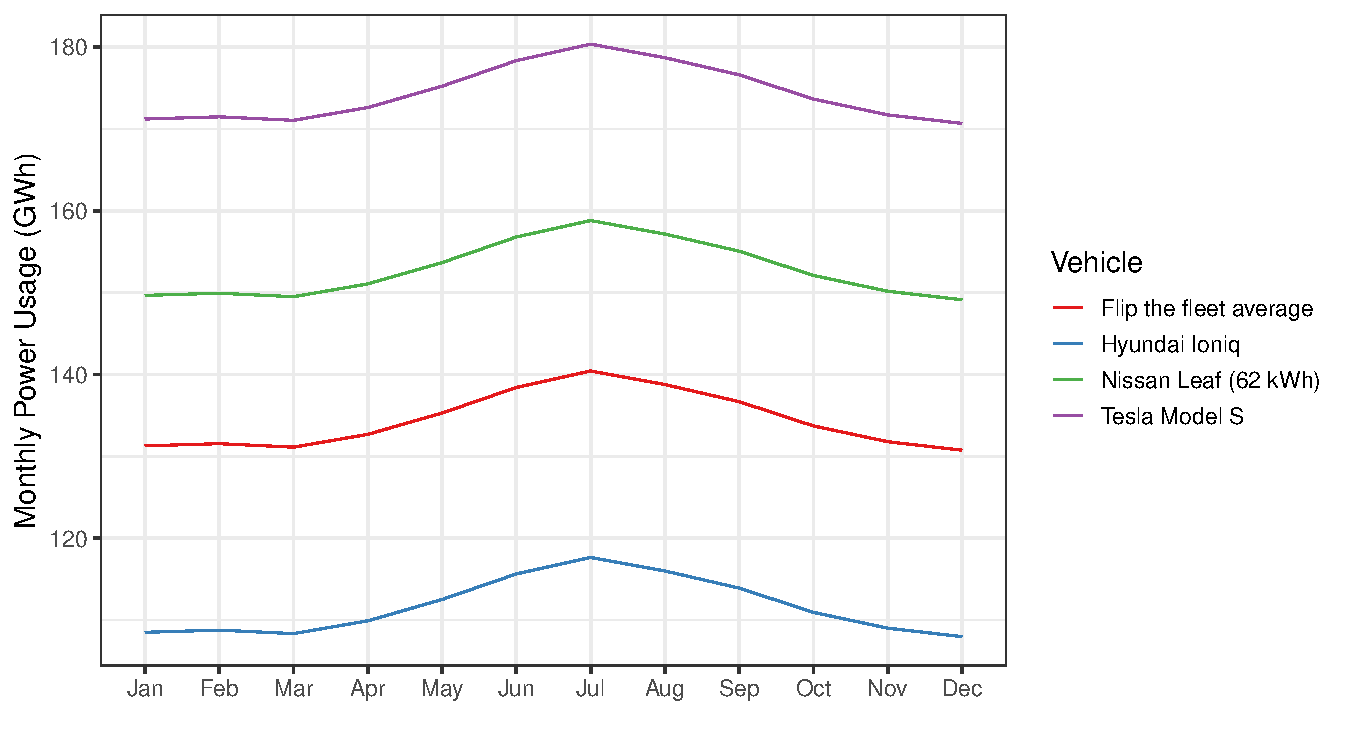
\includegraphics{summary_week4_files/figure-latex/vehicle_power_usage_auck-1.pdf}
\caption{2019 VKT 100\% EV Case Auckland Total Power Usage Scenarios by
Vehicle Fleet Model Makeup\label{fig:vehicle_power_usage_auck}}
\end{figure}

Combining the regional consumption used to plot figure
\ref{fig:vehicle_consum} with the 2019 VKT number we can get an expected
power usage for all of NZ and also for each VKT region. Figure
\ref{fig:vehicle_power_usage} shows with a 100\% EV penetration and an
EV fleet comparable to the Flip the Fleet, the monthly power usage for
all of NZ goes from 425 GWh minimum in the summer to 463 GWh maximum
power usage in the winter. If the fleet consisted of heavier less
efficient vehicles like the Tesla Model S this would increase to 551 GWh
minimum in the summer to 588 GWh maximum power usage in the winter.
Figure \ref{fig:vehicle_power_usage_auck} shows with a 100\% EV
penetration and an EV fleet comparable to the Flip the Fleet, the
monthly power usage of Auckland goes from 131 GWh minimum in the summer
to 140 GWh maximum power usage in the winter. If the fleet consisted of
heavier less efficient vehicles like the Tesla Model S this would
increase to 171 GWh minimum in the summer to 180 GWh maximum power usage
in the winter.

\begin{figure}
\centering
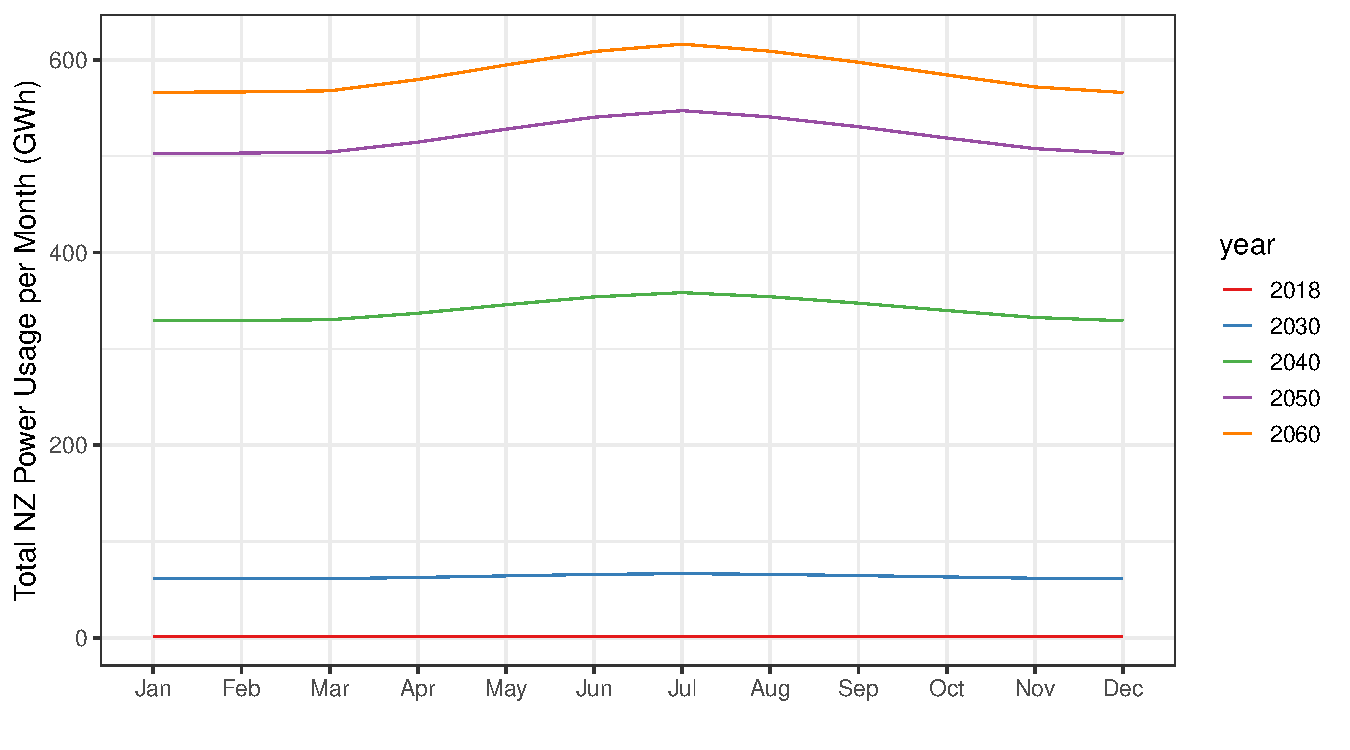
\includegraphics{summary_week4_files/figure-latex/kea_power_usage-1.pdf}
\caption{NZ EVs Power Usage per Month using EECAs kea VKT and Flip the
Fleets Average Consumption\label{fig:kea_power_usage}}
\end{figure}

\begin{figure}
\centering
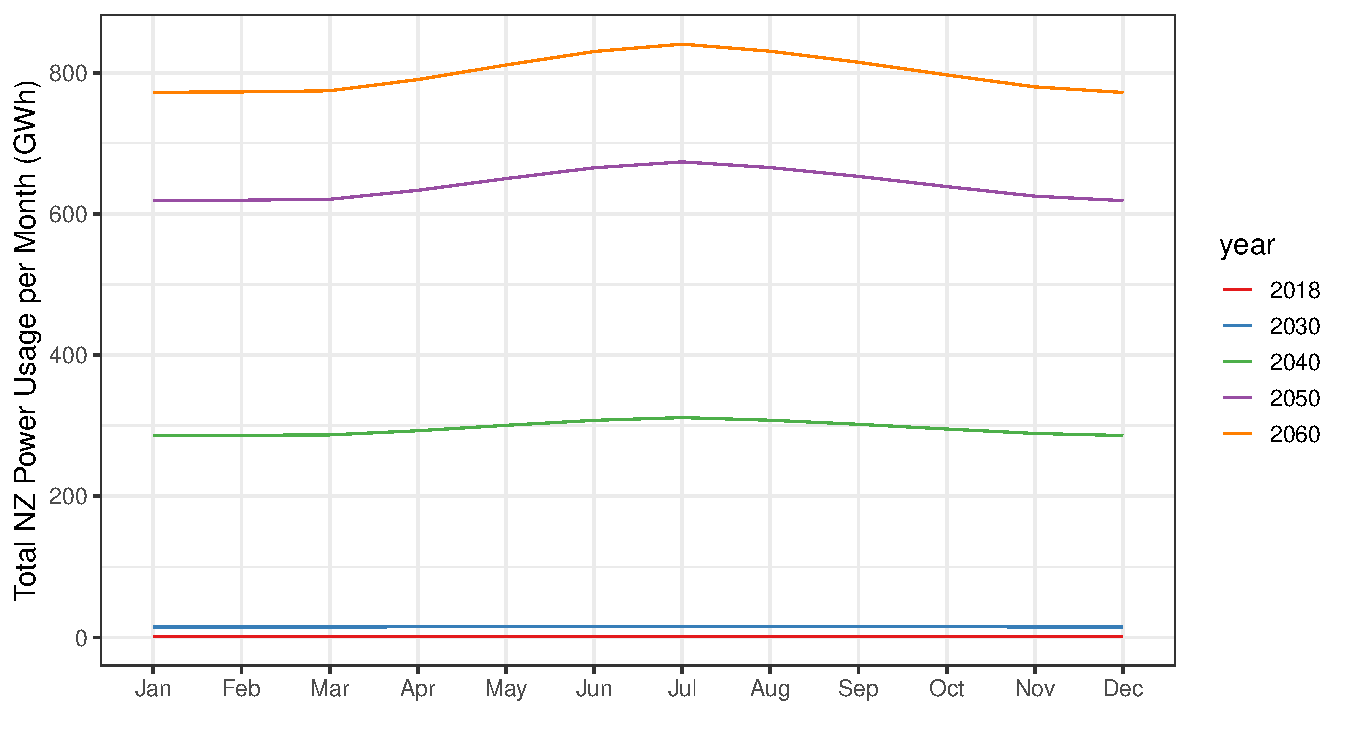
\includegraphics{summary_week4_files/figure-latex/tui_power_usage-1.pdf}
\caption{NZ EVs Power Usage per Month using EECAs Tui VKT and Flip the
Fleets Average Consumption\label{fig:tui_power_usage}}
\end{figure}

This consumption used to plot figure \ref{fig:vehicle_consum} can also
be combined with the EECA's Times Models expected EV VKT we can get an
estimate for power usage used each month of the year based on the kea
(Fig \ref{fig:kea_power_usage}) and tui (Fig \ref{fig:tui_power_usage})
scenario VKT and Flip the Fleet consumption data.

\begin{thebibliography}{9}
\bibitem{ev_range}
\textit{To what degree does temperature impact EV range?}
\\\texttt{\url{https://www.geotab.com/blog/ev-range/}}
\bibitem{ev_highway}
\textit{Why is the range of an EV less on the freeway than the city?}
\\\texttt{\url{https://evcentral.com.au/why-is-the-range-of-an-ev-less-on-the-freeway-than-the-city/}}
\bibitem{HDD_est}
\textit{Bayesian estimation of a building's base temperature for the calculation of heating degree-days}
\\\texttt{https://www.sciencedirect.com/science/article/abs/pii/S0378778816312907}
\bibitem{NZTA_VKT}
\textit{NZTA VKT data website}
\\\texttt{https://www.transport.govt.nz/statistics-and-insights/fleet-statistics/vehicle-kms-travelled-vkt-2/}
\bibitem{times_model}
\textit{ECCA Times Model}
\\\texttt{https://www.eeca.govt.nz/insights/data-tools/new-zealand-energy-scenarios-times-nz/}
\end{thebibliography}

\end{document}
